\chapter{Elasticity in port-Hamiltonian form}

\epigraph{I try not to break the rules but merely to test their elasticity.}{\textit{Bill Veeck}}
\minitoc

\lettrine{\color{theme}{C}}ontinuum mechanics is the mathematical description of how materials behave kinematically under external excitations. In this framework, the microscopic structure of a material body is neglected and a macroscopic viewpoint, that describes the body as a continuum, is adopted. This leads to a PDE based model. In this chapter, the general linear elastodynamics problem is recalled. A suitable port-Hamiltonian formulation is then derived.

\section{Continuum mechanics}
In this section, the main concepts behind a deformable continuum are briefly recalled following \cite{lee2012mixed}. For a detailed discussion on this topic, the reader may consult \cite{abeyaratne2012notes,landau2012elasticity}. 

\subsection{Non-linear formulation of elasticity}

The bounded region of $\mathbb{R}^d, \; d\in \{2, 3\}$ occupied by a solid is called configuration. The reference configuration $\Omega$ is the domain that a body occupies at the initial state. To describe how the body deforms in time the deformation map $\bm\Phi: \Omega \times [0, T_f] \rightarrow \Omega' \subset \mathbb{R}^d$ is introduced. This map is differentiable and orientation preserving, and the image of $\Omega$ under $\bm\Phi(\cdot, t) \; \forall t \in [0, T_f]$ is called the deformed configuration $\Omega_t$. Given a specific point in the reference frame its image is denoted by $\bm{y} = \bm{\Phi}(\bm{x}, t)$. The gradient of the deformation map is called the deformation gradient $\bm{F}:=\nabla_x\bm{\Phi} = \diffp{\bm{y}}{\bm{x}}$. A rigid deformation maps a point $\bm{x} \in \Omega \rightarrow \bm{A}(t) \bm{x} + \bm{b}(t)$, where $\bm{A}(t)$ is an orthogonal matrix and $\bm{b}(t) \in \mathbb{R}^d$ a vector. A differentiable deformation map $\bm\Phi$ is a rigid deformation iff $\bm{F}^\top \bm{F} - \bm{I} = 0$,  where $\bm{I}$ is the identity in $\mathbb{R}^{d\times d}$ (for the proof see \cite{ciarlet1988mathematical}, page 44). For this reason, a suitable measure of the deformation is the Green-St.Venant strain tensor $\frac{1}{2} (\bm{F}^\top \bm{F} - \bm{I})$.  \\
A quantity of interest is the displacement $\bm{u}: \Omega \times [0, T_f] \rightarrow \mathbb{R}^d$ with respect to the reference configuration. It is defined as $\bm{u}(\bm{x}, t) = \bm{\Phi}(\bm{x}, t) - \bm{x}$. The gradient of the displacement verifies $\nabla_x \bm{u} = \bm{F} - \bm{I}$. The strain tensor can now be written in terms of the displacement
\begin{equation*}
\begin{aligned}
\frac{1}{2} (\bm{F}^\top \bm{F} - \bm{I}) &= \frac{1}{2}\left[(\nabla_x \bm{u} + \bm{I})^\top (\nabla_x \bm{u} + \bm{I}) - \bm{I}\right] \\
&= \frac{1}{2}\left[\nabla_x \bm{u} + (\nabla_x \bm{u})^\top + (\nabla_x \bm{u})^\top (\nabla_x \bm{u})\right],
\end{aligned}
\end{equation*}
or in components 
\begin{equation*}
\frac{1}{2} ({F}_{ik}^\top {F}_{kj} - {I}_{ij}) = \frac{1}{2} \left(\diffp{u_i}{x_j} + \diffp{u_j}{x_i} + \diffp{u_i}{x_j}\diffp{u_j}{x_i}\right).
\end{equation*}

To state the balance laws the actual deformed configuration is considered. The linear and angular momenta in a subdomain $\omega_t \subset \Omega_t$ are computed as 
\begin{equation*}
\int_{\omega_t} \rho \, \bm{v} \d{\omega_t}, \quad\text{and}\quad \int_{\omega_t} \rho \, \bm{y} \times \bm{v} \d{\omega_t},
\end{equation*}
where $\rho$ is the mass density and the velocity $\bm{v} = \frac{D\bm{u}}{Dt}(\bm{y},t) = \diffp{\bm{u}}{t}(\bm{x},t)$ is the material time derivative of the displacement (see \cite[Chapter 1]{abeyaratne2012notes}).  Let $\omega_{t, 1},\, \omega_{t, 2}$ be two subregions in a deformed continuum $\Omega_t$ with contacting surface $S_{12}$. There is a force acting on this surface for a continuum that is called stress vector. If $\bm{n}$ is the outward normal at $\bm{y}$ on $S_{12}$ with respect to $\omega_{t, 1}$, then the surface force that $\omega_{t, 1}$ exerts on $\omega_{t, 2}$ is denoted by $\bm{t}(\bm{y}, \bm{n}) \in \mathbb{R}^d$. By the Newton third law, the surface force that $\omega_{t, 2}$ applies on $\omega_{t, 1}$ is given by $\bm{t}(\bm{y}, -\bm{n}) = - \bm{t}(\bm{y}, \bm{n})$. It is assumed that the linear and angular momentum balances hold for any subregion $\omega_t \in \Omega_t$ 
\begin{align*}
	\diff{}{t} \int_{\omega_t} \rho \bm{v} \d{\omega_t} &= \int_{\partial \omega_t} \bm{t}(\bm{y}, \bm{n}) \d{S} + \int_{\omega_t} \bm{f} \d{\omega_t}, \\
	\diff{}{t} \int_{\omega_t} \rho\bm{y} \times \bm{v} \d{\omega_t} &= \int_{\partial \omega_t} \bm{y} \times \bm{t}(\bm{y}, \bm{n}) \d{S} + \int_{\omega_t} \bm{y} \times \bm{f} \d{\omega_t}, \\
\end{align*}
where $\partial \omega_t$ stands for the boundary surface of the subdomain $\omega_t$, $\bm{n}$ is the outward normal to the surface $\partial\omega_t$ and $\bm{f}$ represents an exterior body force. The following theorem characterizes the stress vector (see \cite[Chapter 2]{ciarlet1988mathematical}):

\begin{theorem}[Cauchy’s theorem]
If the linear and angular momenta balances hold, then there exists a matrix-valued function $\bm{\Sigma}$ from $\Omega_t$ to $\mathbb{S}$ such
that $\bm{t}(\bm{y}, \bm{n}) = \bm{\Sigma}(\bm{y}) \bm{n}, \; \forall \bm{y} \in \Omega_t$ where the right-hand side is the matrix-vector multiplication.
\end{theorem}
The set $\mathbb{S}=\mathbb{R}^{d\times d}_{\mathrm{sym}}$ denotes the field of symmetric matrices in $\mathbb{R}^{d\times d}$. The symmetry of the stress tensor $\bm{\Sigma}$ is due to the balance of angular momentum. The divergence theorem can then be applied
\begin{equation*}
\int_{\partial \omega_t} \bm{\Sigma} \, \bm{n} \d{S} = \int_{\omega_t} \nabla_y \cdot\bm{\Sigma} \d{\omega_t},
\end{equation*}
where $\nabla_y \cdot$ is the tensor divergence with respect to the deformed configuration, $\nabla_y \cdot\bm{\Sigma} = \sum_{i=1}^{d}\diffp{\Sigma_{ij}}{y_i}$.
Because the considered subregion $\omega_t$ is arbitrary, using the linear balance momentum and the conservation of mass, the following PDE is found
\begin{equation*}
	\rho \frac{D\bm{v}}{Dt} - \nabla_y \cdot{\bm{\Sigma}} = \bm{f}, \qquad \bm{y} \in \Omega_t.
\end{equation*}
This equation is written with respect to the deformed configuration $\Omega_t$. For a detailed derivation of this equation the reader may consult \cite[Chapter 4]{abeyaratne2012notes}. To obtain a closed formulation, the constitutive law, namely the link between the stress tensor $\bm{\Sigma}$ and the strain tensor $\frac{1}{2} (\bm{F}^\top \bm{F} - \bm{I})$, has to be introduced. In the next section such relation will be discussed for the case of linear elasticity.

\subsection{The linear elastodynamics problem}\label{sec:linElas}
Whenever deformations are small, $\norm{\nabla_x\bm{u}} \ll 1$, then the reference and deformed configurations are almost indistinguishable $\bm{y} = \bm{x} + \bm{u} = \bm{x}  + O(\nabla_x\bm{u}) \approx \bm{x}$. This allows writing the linear momentum balance in the reference configuration
\begin{equation*}
	\rho \diffp{\bm{v}}{t}(\bm{x, t}) - \Div \bm\Sigma(\bm{x}, t) = \bm{f}, \qquad \bm{x} \in \Omega.
\end{equation*}
The material derivative simplifies to a partial one. The operator $\Div$ is the divergence of a tensor field with respect to the reference configuration (see Appendix \ref{app:math} for a description of the differential operators)
\begin{equation*}
\Div \bm\Sigma(\bm{x}, t) = \nabla_x \cdot \bm\Sigma(\bm{x}, t) = \left(\sum_{i=1}^{d}\diffp{\Sigma_{ij}}{x_i}\right)_{1 \leq j \leq d}.
\end{equation*}
Furthermore, the non-linear terms in the Green-St. Venant strain tensor can be dropped
\begin{equation*}
\frac{1}{2} (\bm{F}^\top \bm{F} - \bm{I}) = \frac{1}{2}\left[\nabla_x \bm{u} + (\nabla_x \bm{u})^\top + (\nabla_x \bm{u})^\top (\nabla_x \bm{u})\right]
\approx \frac{1}{2}\left[\nabla_x \bm{u} + (\nabla_x \bm{u})^\top\right].
\end{equation*}
The linearized strain tensor (also called infinitesimal strain tensor) is the symmetric gradient of the displacement
\begin{equation}
\bm{\varepsilon} := \Grad\bm{u}, \where \Grad\bm{u} = \frac{1}{2}\left[\nabla_x \bm{u} + (\nabla_x \bm{u})^\top\right].
\end{equation}

To obtain a closed system of equations, it is now necessary to characterize the relation between stress and strain. This relation is normally called \textit{constitutive law}. In the following, the particular case of elastic materials is considered. These materials are able to return back to their original size and shapes after forces are removed. For this class of materials, the stress tensor is solely determined from the deformed configuration at a given time (Hooke's law)
\begin{equation*}
\bm{\Sigma}(\bm{x}) = \bm{\mathcal{D}}(\bm{x}) \, \bm{\varepsilon}(\bm{u}(\bm{x})).
\end{equation*}
The \textit{stiffness tensor} or \textit{elasticity tensor} $\bm{\mathcal{D}} : \mathbb{S} \rightarrow \mathbb{S}$ is a rank 4 tensor that is symmetric positive definite and uniformly bounded above and below. Because of symmetry, its components satisfy
\begin{equation*}
\mathcal{D}_{ijkl} = \mathcal{D}_{jikl} = \mathcal{D}_{klij}.
\end{equation*}
From the uniform boundedness of $\bm{\mathcal{D}}$, the map
$\bm{\mathcal{D}}: L^2 (\Omega, \mathbb{S}) \rightarrow L^2 (\Omega, \mathbb{S})$ is a symmetric positive definite bounded linear operator ($L^2 (\Omega, \mathbb{S})$ is the space of square-integrable symmetric tensor-valued functions). The compliance tensor $\bm{\mathcal{C}}$ is defined by $\bm{\mathcal{C}} = \bm{\mathcal{D}}^{-1}$ . Thus $\bm{\mathcal{C}} : \mathbb{S} \rightarrow \mathbb{S}$ is as well symmetric positive definite and uniformly bounded above and below. An isotropic
elastic medium has the same kinematic properties in any direction and at each point. If an elastic medium is isotropic, then the stiffness and compliance tensors assume the form
\begin{equation}
\bm{\mathcal{D}}(\cdot) = 2\mu (\cdot) + \lambda \Tr(\cdot)\bm{I}, \qquad \bm{\mathcal{C}}(\cdot) = \frac{1}{2\mu}\left[(\cdot) - \frac{\lambda}{2\mu + d\lambda}\Tr(\cdot)\bm{I}\right], \qquad d= \{2,3\},
\end{equation}
where  $\Tr$ is the trace operator and the positive scalar functions $\mu, \lambda$, defined on $\Omega$, are called the Lam\'e coefficients. In engineering applications it is easier to compute experimentally two other parameters: the Young modulus $E$ and  Poisson's ratio $\nu$. Those are expressed in terms of the Lam\'e  coefficients as 
\begin{equation}
\nu =\frac{\lambda}{2(\lambda +\mu)}, \qquad 
E=\frac{\mu (3\lambda +2\mu)}{\lambda +\mu},
\end{equation}
and conversely
\begin{equation}
\lambda =\frac {E \nu }{(1+\nu )(1-2\nu )}, \qquad
\mu = \frac{E}{2(1+\nu)}.
\end{equation}
The stiffness and compliant tensor are expressed as
\begin{align}
	\bm{\mathcal{D}}(\cdot) &= \frac{E}{1+\nu} \left[(\cdot) + \frac{\nu}{1-2\nu}\Tr(\cdot)\bm{I}\right], \label{eq:stiff3D} \vspace{3pt}\\
	\bm{\mathcal{C}}(\cdot) &= \frac{1+\nu}{E}\left[(\cdot) - \frac{\nu}{1+\nu(d-2)}\Tr(\cdot)\bm{I}\right].
\end{align}
The linear elastodynamics problem is formulated through a vector-valued PDE
\begin{equation}\label{eq:lin_elastodyn}
\rho \diffp[2]{\bm{u}}{t} - \Div(\bm{\mathcal{D}} \Grad \bm{u}) = \bm{f}.
\end{equation}  
The classical elastodynamics problem is expressed considering the displacement $\bm{u}$ as the unknown. This PDE goes together with appropriate boundary conditions that will be specified in \ref{sec:pHelas}.



\section{Port-Hamiltonian formulation of linear elasticity}\label{sec:pHelas}

In this section a port-Hamiltonian formulation for elasticity is deduced from the classical elastodynamics problem. It must be highlighted that already in the seventies a purely hyperbolic formulation for elasticity was detailed \cite{hughes1978classical}. The missing point is the clear connection with the theory of Hamiltonian PDEs. An Hamiltonian formulation can be found in \cite[Chapter 16]{grinfield2015}, but without any connection to the concept of Stokes-Dirac structure induced by the underlying geometry. \\

\subsection{Energy and co-energy variables}
Consider an open connected set $\Omega \subset \mathbb{R}^d, \; d \in \{2,3\}$. The displacement within a deformable continuum is given by Eq. \eqref{eq:lin_elastodyn}. 
\begin{equation}
\rho \diffp[2]{\bm{u}}{t} - \Div(\bm{\mathcal{D}} \Grad \bm{u}) =0, \qquad \bm{x} \in \Omega.
\end{equation}
The contribution of the body force $\bm{f}$ has been removed for ease of presentation. To derive a pH formulation, the total energy, that includes the kinetic and  deformation energy, is needed
\begin{equation}
	H = \energy{\rho \norm{\partial_t \bm{u}}^2 + \bm{\Sigma} \cddot \bm{\varepsilon}}.
\end{equation}
The notation $\bm{A}\cddot \bm{B} = \Tr(\bm{A}^\top\bm{B}) = \sum_{i, j} A_{ij} B_{ij}$ denotes the tensor contraction. Recall that $\bm{\varepsilon}= \Grad{\bm{u}}$ and $\bm{\Sigma}=\bm{\mathcal{D}}\bm{\varepsilon}$. The energy variables are then the linear momentum and the deformation field
\begin{equation*}
\bm{\alpha}_v = \rho \bm{v}, \qquad \bm{A}_{\varepsilon} = \bm{\varepsilon},
\end{equation*}
where $\bm{v}:= \partial_t \bm{u}$. The Hamiltonian can be rewritten as a quadratic functional in the energy variables
\begin{equation}
H = \energy{\frac{1}{\rho} \bm{\alpha}_v^2 + (\bm{\mathcal{D}} \bm{A}_{\varepsilon}) \cddot  \bm{A}_{\varepsilon}}.
\end{equation}
The co-energy variables are given by
\begin{equation}
\bm{e}_v := \diffd{H}{\bm{\alpha}_v} = \bm{v}, \qquad \bm{E}_\varepsilon := \diffd{H}{\bm{A}_{\varepsilon}} = \bm{\Sigma}.
\end{equation}  

The tensor-valued co-energy $\bm{E}_\varepsilon$ is obtained by taking the variational derivative with respect to a tensor.
\begin{proposition}\label{prop:varder_tens}
	The variational derivative of the Hamiltonian with respect to the strain tensor is the stress tensor $\delta_{\bm{A}_{\varepsilon}}H = \bm{\Sigma}$.
	\begin{proof}
		Let $\mathbb{S}: \mathbb{R}^{d\times d}_{\text{sym}}$ be the space of symmetric tensor and  $L^2(\Omega, \mathbb{S})$ the space of the square-integrable symmetric tensors endowed with the tensor contraction as inner product
		\begin{equation}\label{eq:normL2sym}
		\inner[L^2(\Omega, \mathbb{S})]{\bm{A}}{\bm{B}} = \int_{\Omega} \bm{A} \cddot \bm{B} \d\Omega. 
		\end{equation}
		The contribution due to the deformation part in Hamiltonian is given by:		\begin{equation*}
		H_{\mathrm{def}}(\bm{A}_{\varepsilon}) = \frac{1}{2} \int_{\Omega} (\bm{\mathcal{D}} \bm{A}_{\varepsilon}) \cddot \bm{A}_{\varepsilon}  \; \d\Omega. 
		\end{equation*}
		A variation $\bm{\Delta}\bm{A}_{\varepsilon}$ of the strain tensor with respect to a given value $\bar{\bm{A}}_{\varepsilon}$ leads to:
		\begin{align*}
		H_{\mathrm{def}}(\bar{\bm{A}}_{\varepsilon} + \eta \bm{\Delta}\bm{A}_{\varepsilon}) = &+\frac{1}{2} \int_{\Omega} (\bm{\mathcal{D}} \bar{\bm{A}}_{\varepsilon}) \cddot \bar{\bm{A}}_{\varepsilon} \; \d\Omega \\
		&+ \eta \frac{1}{2} \int_{\Omega} \left\{ (\bm{\mathcal{D}} \bar{\bm{A}}_{\varepsilon}) \cddot \bm{\Delta}\bm{A}_{\varepsilon}
		+ (\bm{\mathcal{D}} \bm{\Delta}\bm{A}_{\varepsilon}) \cddot \bar{\bm{A}}_{\varepsilon}\right\}\; \d\Omega  + O(\eta^2).
		\end{align*}

		The term $(\bm{\mathcal{D}} \bm{\Delta}\bm{A}_{\varepsilon}) \cddot \bar{\bm{A}}_{\varepsilon}$ can be further rearranged using the symmetry of $\bm{\mathcal{D}}$ and the commutativity of the tensor contraction
		\begin{equation*} 
		(\bm{\mathcal{D}} \bm{\Delta}\bm{A}_{\varepsilon}) \cddot \bar{\bm{A}}_{\varepsilon} = (\bm{\mathcal{D}} \bar{\bm{A}}_{\varepsilon}) \cddot \bm{\Delta}\bm{A}_{\varepsilon},
		\end{equation*}
		so that 
		\begin{equation*}
		H_{\mathrm{def}}(\bar{\bm{A}}_{\varepsilon} + \eta \bm{\Delta}\bm{A}_{\varepsilon}) = \frac{1}{2} \int_{\Omega} (\bm{\mathcal{D}} \bar{\bm{A}}_{\varepsilon}) \cddot \bar{\bm{A}}_{\varepsilon} \; \d\Omega + \eta \int_{\Omega} (\bm{\mathcal{D}} \bar{\bm{A}}_{\varepsilon}) \cddot \bm{\Delta}\bm{A}_{\varepsilon}\; \d\Omega  + O(\eta^2). 
		\end{equation*}
		By definition of  variational derivative it can be written:
		\begin{equation*}H_{\mathrm{def}}(\bar{\bm{A}}_{\varepsilon} + \eta \bm{\Delta}\bm{A}_{\varepsilon}) = H_{\mathrm{def}}(\bar{\bm{A}}_{\varepsilon}) + \eta \inner[L^2(\Omega, \mathbb{S})]{\diffd{H}{\bm{A}_{\varepsilon}}}{\bm{\Delta}\bm{A}_{\varepsilon}} + O(\eta^2), \end{equation*}
		
		Then, by identification 
		\begin{equation*}
		\diffd{H_{\mathrm{def}}}{\bm{A}_{\varepsilon}} = \bm{\mathcal{D}} \bar{\bm{A}}_{\varepsilon} = \bm{\Sigma}.
		\end{equation*}
		Since the Hamiltonian is separable then $\delta_{\bm{A}_{\varepsilon}}{H_{\mathrm{def}}} =\delta_{\bm{A}_{\varepsilon}} H$, leading to the final result.
	\end{proof}
\end{proposition}

\subsection{Final system and associated Stokes-Dirac structure}

It is now possible to state the final pH form
\begin{equation}
\diffp{}{t}
\begin{pmatrix}
\bm{\alpha}_v \\
\bm{A}_\varepsilon
\end{pmatrix} = 
\begin{bmatrix}
\bm{0} & \Div \\
\Grad & \bm{0} \\
\end{bmatrix}
\begin{pmatrix}
\bm{e}_v \\
\bm{E}_\varepsilon
\end{pmatrix}.
\end{equation}
The first equation of the system is the conservation of linear momentum. The second represents a compatibility condition 
\begin{equation}\label{eq:compderElas}
\begin{aligned}
\partial_t {\bm{A}_\varepsilon} &= \Grad(\bm{e}_v), \\
\partial_t\bm{\varepsilon} &= \Grad(\bm{v}), \\
\partial_t \Grad \bm{u} &= \Grad(\partial_t \bm{u}). \\
\end{aligned}
\end{equation}

Assuming that $\bm{u} \in C^2$, higher order derivatives commute (Clairaut's theorem). Hence, the equation is verified. The following theorem ensures the differential operator is formally skew-adjoint (one can also find this result in the recent article \cite[Lemma 3.3]{pauly2020elasticity}, available as arXiv preprint). 

\begin{theorem}\label{th:adjDiv}
	The formal adjoint of the tensor divergence $\mathrm{Div}$ is $- \mathrm{Grad}$, the opposite of the symmetric gradient.
	\begin{proof}
		We denote by $\mathbb{V} = \mathbb{R}^{d}$ the space of vector field in $\mathbb{R}^{d}$ and by $\mathbb{S} = \mathbb{R}^{d\times d}$ the space of symmetric tensor field in $\mathbb{R}^{d\times d}$. Let us consider the Hilbert space of the square-integrable symmetric tensors $L^2(\Omega, \mathbb{S})$ with scalar product defined in \eqref{eq:normL2sym}. Moreover consider the Hilbert space of the square-integrable vector function $L^2(\Omega, \mathbb{V})$, endowed with the usual scalar product
		\begin{equation*}
		\left\langle \bm{a} , \bm{b} \right\rangle_{L^2(\Omega, \mathbb{V})} = \int_{\Omega}  \bm{a} \cdot \bm{b} \; \d\Omega. 
		\end{equation*}
		Let us consider the tensor divergence operator defined as:
		\begin{equation*}
		\begin{aligned}
		\Div: \; L^2(\Omega, \mathbb{S})& \rightarrow L^2(\Omega, \mathbb{V}), \\
		\bm{\Psi}& \rightarrow \Div\bm{\Psi} = \bm{\psi}, \\
		\end{aligned}
		\qquad \text{with } \psi_j = \mathrm{div}(\Psi_{ij}) = \sum_{i = 1}^d \diffp{\Psi_{ij}}{x_i}.
		\end{equation*}
		We try to identify $\Div{}^*$
		\begin{equation*}
		\begin{aligned}
		\Div{}^*: \; L^2(\Omega, \mathbb{V}) & \rightarrow L^2(\Omega, \mathbb{S}), \\
		\bm{\phi}& \rightarrow  \Div{}^* \bm{\phi} = \bm{\Phi}, \\
		\end{aligned}
		\end{equation*}
		such that \begin{equation*}
		\inner[{L^2(\Omega, \mathbb{V})}]{\Div \bm{\Psi}}{\bm{\phi}}  = \inner[{L^2(\Omega, \mathbb{S})}]{\bm{\Psi}} {\Div{}^* \bm{\phi}},
		\begin{aligned} \qquad
		&\forall \bm{\Psi} \in \Dom(\Div) \subset L^2(\Omega, \mathbb{S}), \\
		&\forall \bm{\phi} \in \Dom(\Div{}^*) \subset L^2(\Omega, \mathbb{V}).
		\end{aligned}
		\end{equation*}
		Now let us take $\bm{\Psi} \in {C}_0^1(\Omega, \mathbb{S}) \subset \mathrm{Domain}(\Div)$ the space of differentiable symmetric tensors with compact support in~$\Omega$. Additionally $\bm{\phi}$ will belong to ${C}_0^1(\Omega, \mathbb{V}) \subset \mathrm{Dom}(\Div{}^*)$, the space of differentiable vector functions with compact support in~$\Omega$. Then
		\begin{equation*}
		\begin{aligned}
		\left\langle \Div\bm{\Psi} , \bm{\phi} \right\rangle_{L^2(\Omega, \mathbb{V})} &= \int_{\Omega}  \bm{\psi} \cdot \bm{\phi} \; \d\Omega, \\
		&= \int_{\Omega} \sum_{i=1}^d \sum_{j=1}^d \diffp{\Psi_{ij}}{x_i} \phi_j \; \d\Omega,  \\ 
		&= - \int_{\Omega} \sum_{i=1}^d \sum_{j=1}^d \Psi_{ij} \diffp{\phi_j}{x_i} \; \d\Omega\,, \qquad &\text{since the functions vanish at the boundary,}\\
		&= - \int_{\Omega} \sum_{i=1}^d \sum_{j=1}^d \Psi_{ij} {F}_{ij} \;\d\Omega,  \qquad &\where {F}_{ij} = \diffp{\phi_j}{x_i},\\
		&= - \left\langle \bm{\Psi} , \bm{F} \right\rangle_{L^2(\Omega, \mathbb{S})},  \qquad &\bm{F} = \grad{\bm\phi}.
		\end{aligned}	 
		\end{equation*}
		But in this latter case, it could not  be stated that $\bm{F} \in L^2(\Omega, \mathbb{S})$. Now, since  $\bm{\Psi} \in L^2(\Omega, \mathbb{S})$, $\Psi_{ji}=\Psi_{ij}$,  thus the last equality can be further decomposed as
		
		\begin{equation*} \sum_{i,j}\Psi_{ij} \diffp{\phi_j}{x_i} = \sum_{i,j}\Psi_{ij} \frac{1}{2} \left(\diffp{\phi_i}{x_j} + \diffp{\phi_j}{x_i}  \right) = 	\sum_{i,j} \Psi_{ij} {\Phi}_{ij}, \qquad \text{with } {\Phi}_{ij}:= \frac{1}{2} \left(\diffp{\phi_i}{x_j} + \diffp{\phi_j}{x_i}  \right).
		\end{equation*}
		Thus $\bm{\Phi}=\Grad \bm{\phi} \in L^2(\Omega, \mathbb{S})$ and it can be stated that:
		\begin{align*}
		\inner[L^2(\Omega, \mathbb{V})]{\Div\bm{\Psi}}{\bm{\phi}} &= - \int_{\Omega} \sum_{i,j} \Psi_{ij} \frac{1}{2} \left(\diffp{\phi_i}{x_j} + \diffp{\phi_j}{x_i}  \right) \;\d\Omega \\
		&= - \int_{\Omega} \sum_{i,j} \Psi_{ij} \Phi_{ij} \;\d\Omega = \inner[L^2(\Omega, \mathbb{S})]{\bm{\Psi}}{-\Grad \bm{\phi}}.
		\end{align*}

		It can be concluded that the formal adjoint of $\Div$ is $\Div{}^* = -\Grad$.
	\end{proof}
\end{theorem}

The boundary values are then found by evaluating the energy rate
\begin{equation}\label{eq:enrateElas}
\begin{aligned}
\dot{H} &= \int_{\Omega} \left\{ \bm{e}_v \cdot \partial_t \bm\alpha_v + \bm{E}_\varepsilon \cddot \partial_t \bm{A}_\varepsilon \right\} \d\Omega, \\
&= \int_{\Omega} \left\{\bm{e}_v \cdot \Div \bm{E}_\varepsilon + \bm{E}_\varepsilon \cddot \Grad \bm{e}_v \right\}\d\Omega,\\
&= \int_{\Omega} \div(\bm{E}_\varepsilon \, \bm{e}_v) \d\Omega, \qquad &\text{Stokes theorem (see  Appendix \ref{app:math} Eq. \eqref{eq:intbypartsSymTens}}), \\
&= \int_{\partial \Omega} \bm{e}_v \cdot (\bm{E}_\varepsilon\bm{n}) \d{S} = \inner[L^2(\partial\Omega, \bbR^d)]{\bm{e}_v}{\bm{E}_\varepsilon \, \bm{n}}.
\end{aligned}
\end{equation}

\begin{figure}
\centering
\includegraphics[width=0.4\textwidth]{part_2/bc_elas2D.eps}
\caption{A 2D continuum with Neumann and Dirichlet boundary conditions}
\label{fig:bc_elas2D}
\end{figure}
The imposition of the velocity field along the boundary $\bm{e}_v = \partial_t \bm{u}$ corresponds to a Dirichlet condition. Setting $\bm{E}_\varepsilon \, \bm{n} = \bm{\Sigma} \,  \bm{n} = \bm{t}$ (the traction) corresponds to a Neumann condition. Consider a partition of the boundary $\partial\Omega = \overline{\Gamma}_N \cup \overline{\Gamma}_D$ and $\Gamma_N \cap \Gamma_D =  \{\emptyset\}$, where a Dirichlet and a Neumann condition applies on the open subset $\Gamma_D$ and $\Gamma_N$ respectively (see Fig. \ref{fig:bc_elas2D}). Then the final pH formulation reads

\begin{equation}\label{eq:pHsysElas}
\begin{aligned}
\displaystyle
\diffp{}{t}
\begin{pmatrix}
\bm{\alpha}_v \\
\bm{A}_\varepsilon
\end{pmatrix} &= \underbrace{
\begin{bmatrix}
\bm{0} & \Div \\
\Grad & \bm{0} \\
\end{bmatrix}}_{\mathcal{J}}
\begin{pmatrix}
\bm{e}_v \\
\bm{E}_\varepsilon
\end{pmatrix}, \vspace{3pt}\\
\bm{u}_\partial &= \underbrace{
	\begin{bmatrix}
	\bm\gamma_{0}^{\Gamma_D} & \bm{0} \\
	\bm{0} & \bm\gamma_n^{\Gamma_N} \\
	\end{bmatrix}}_{\mathcal{B}_\partial} \begin{pmatrix}
\bm{e}_v \\
\bm{E}_\varepsilon
\end{pmatrix}, \vspace{3pt}\\
\bm{y}_\partial &= \underbrace{
\begin{bmatrix}
\bm{0} & \bm\gamma_{n}^{\Gamma_D} \\
\bm\gamma_0^{\Gamma_N} & \bm{0} \\
\end{bmatrix}}_{\mathcal{C}_\partial}
\begin{pmatrix}
\bm{e}_v \\
\bm{E}_\varepsilon
\end{pmatrix},
\end{aligned}
\end{equation}
where $\bm\gamma_{0}^{\Gamma_*}$ denotes the trace over the set $\Gamma_*$, namely $\bm\gamma_{0}^{\Gamma_*}\bm{e}_v = \bm{e}_v\vert_{\Gamma_*}$. Furthermore, $\bm\gamma_{n}^{\Gamma_*}$ denotes the normal trace over the set $\Gamma_*$, namely $\bm\gamma_{n}^{\Gamma_*}\bm{E}_\varepsilon = \bm{E}_\varepsilon \bm{n}\vert_{\Gamma_*}$.

\begin{remark}\label{rmk:unboundednessBC}
	The boundary operators $\mathcal{B}_\partial, \mathcal{C}_\partial$ in Eq.\eqref{eq:pHsysElas} are unbounded if the co-energy belong to $H^{\Grad}, \; H^{\Div}$ (see conjecture \ref{conj:stdirElas}).
\end{remark}

\begin{conjecture}[Stokes-Dirac structure for elastodynamics] \label{conj:stdirElas}
Let $H^{\Grad}(\Omega, \mathbb{V})$ denote the space of vectors with symmetric gradient in $L^2(\Omega, \mathbb{S})$ and $H^{\Div}  (\Omega, \mathbb{S})$ be the space of symmetric tensors with divergence in $L^2(\Omega, \mathbb{V})$. Consider the following definitions
\begin{align*}
H &:= H^{\Grad}(\Omega, \mathbb{V}) \times H^{\Div}(\Omega, \mathbb{S}), \\
F &:= L^2(\Omega, \mathbb{V}) \times L^2(\Omega, \mathbb{S}), \\
F_\partial &:= L^2(\Gamma_D, \mathbb{V}) \times L^2(\Gamma_N, \mathbb{V}).
\end{align*}

The set 
\begin{equation}
{D}_{\mathcal{J}} = \left\{
\begin{pmatrix}
\bm{f} \\ \bm{f}_\partial \\ \bm{e} \\ \bm{e}_\partial \\
\end{pmatrix}
\vert \;
 \bm{e} \in H, \; \bm{f} = \mathcal{J} \bm{e}, \;\bm{f}_\partial = \mathcal{B}_\partial \bm{e}, \; \bm{e}_\partial = -\mathcal{C}_\partial \bm{e}   \right\},
\end{equation}
where $\bm{e} = (\bm{e}_v,\, \bm{E}_\varepsilon)$ and $\mathcal{J, \, B_\partial, \,  C_\partial}$ are defined in \eqref{eq:pHsysElas}, is a Stokes–Dirac structure with respect to the pairing
\begin{equation}\label{eq:bilinearElas}
\bilprod{(\bm{f}^1, \bm{f}_{\partial}^1, \bm{e}^1, \bm{e}_{\partial}^1)}{(\bm{f}^2, \bm{f}_{\partial}^2, \bm{e}^2, \bm{e}_{\partial}^2)}  := \inner[F]{\bm{e}^1}{\bm{f}^2} + \inner[F]{\bm{e}^2}{\bm{f}^1} + \inner[F_\partial]{\bm{e}_{\partial}^1}{\bm{f}_{\partial}^2} + \inner[F_\partial]{\bm{e}_{\partial}^2}{\bm{f}_{\partial}^1},
\end{equation}
where 
\begin{equation*}
\inner[F_\partial]{(\bm{a}, \, \bm{b})}{(\bm{c}, \, \bm{d})} = \int_{\Gamma_D} \bm{a} \cdot \bm{c} \d{S} + \int_{\Gamma_N} \bm{b} \cdot \bm{d} \d{S}, \quad \bm{a},\ \bm{b},\ \bm{c},\ \bm{d} \in \mathbb{V}. 
\end{equation*}
\end{conjecture}

\begin{remark}[Trace operators and duality pairing for the elastodynamics problem]\label{rmk:duality_elas}
	For linear elastodynamics the integrations by parts formula leads to the following duality pairings \cite[Chapter 1]{boffi2013mixed}
	\begin{equation}\label{eq:duality_elas}
	\inner[L^2(\Omega, \bbS)]{\bm{E}_\varepsilon}{\Grad \bm{e}_v} + \inner[L^2(\Omega, \bbR^d)]{\Div \bm{E}_\varepsilon}{\bm{e}_v} = \inner[H^{-\frac{1}{2}} \times H^{\frac{1}{2}}(\partial\Omega, \bbR^d)]{\bm\gamma_{n}\bm{E}_\varepsilon}{\bm\gamma_{0} \bm{e}_v},
	\end{equation}
	where $H^{\frac{1}{2}}(\partial\Omega, \bbR^d)$ is the space of traces of functions belonging to $H^{\Grad}(\Omega, \bbR^d)$ and $H^{-\frac{1}{2}}(\partial\Omega, \bbR^d)$ is its topological dual.
\end{remark}

\begin{paragraph}{Crucial points to obtain a rigorous proof}
	The crucial point that needs to be elucidated is where the boundary variables live. From Eq. \eqref{eq:duality_elas}, it is clear that when only only one kind of boundary condition is imposed (either Neumann or Dirichlet), these variables belong to the fractional Sobolev spaces $H^{\frac{1}{2}}(\partial\Omega, \mathbb{V}), \, H^{-\frac{1}{2}}(\partial\Omega, \mathbb{V})$ linked by duality with respect to the pivot space $L^2(\partial\Omega, \mathbb{V})$ (cf. Remark \ref{rmk:duality_elas}). This is why an $L^2$ inner product has been assumed as boundary inner product. The partition of the boundary due to the non uniform boundary control complicates the proof, since one has to properly connect the two partitions at their interconnection.
\end{paragraph}

\begin{paragraph}{Elements to support the conjecture}
	A Stokes-Dirac is characterized by the fact that ${D}_{\mathcal{J}} = {D}_{\mathcal{J}}^\perp$. Then one has to show that ${D}_{\mathcal{J}} \subset {D}_{\mathcal{J}}^\perp$ and ${D}_{\mathcal{J}}^\perp \subset {D}_{\mathcal{J}}$. The main steps of Theorem 3.6 in \cite{legorrec2005} (and Proposition \ref{prop:stdir}) are followed here to support the substantiation of the conjecture. The integration by parts formula is applied as in \eqref{eq:enrateElas}. \\
	
	\textit{Step 1}. To show that ${D}_{\mathcal{J}} \subset {D}_{\mathcal{J}}^\perp$, take $(\bm{f}, \, \bm{f}_\partial, \, \bm{e}, \, \bm{e}_\partial) \in {D}_{\mathcal{J}}$. Then
	\begin{align*}
	\bilprod{(\bm{f}, \bm{f}_{\partial}, \bm{e}, \bm{e}_{\partial})}{(\bm{f}, \bm{f}_{\partial}, \bm{e}, \bm{e}_{\partial})} =& 2 \inner[F]{\bm{e}}{\bm{f}} + 2 \inner[F_\partial]{\bm{e}_{\partial}}{\bm{f}_{\partial}}, \\
	=& 2 \inner[F]{\bm{e}}{\mathcal{J}\bm{e}} + 2 \inner[F_\partial]{\bm{e}_{\partial}}{\bm{f}_{\partial}}, \\
	=& + 2 \int_{\Omega} \left\{\bm{e}_v \cdot \Div \bm{E}_\varepsilon + \bm{E}_\varepsilon \cddot \Grad \bm{e}_v \right\}\d\Omega\\
	&- 2 \int_{\Gamma_D} \bm{e}_v \cdot (\bm{E}_\varepsilon \, \bm{n}) \d{S} - 2 \int_{\Gamma_N} \bm{e}_v \cdot (\bm{E}_\varepsilon \, \bm{n}) \d{S}, \\
	=& + 2 \int_{\Omega} \left\{\bm{e}_v \cdot \Div \bm{E}_\varepsilon + \bm{E}_\varepsilon \cddot \Grad \bm{e}_v \right\}\d\Omega\\
	& - 2 \int_{\partial\Omega} \bm{e}_v \cdot (\bm{E}_\varepsilon \, \bm{n}) \d{S},
	= 0, \quad \text{from \eqref{eq:enrateElas}}.
	\end{align*}
	This implies ${D}_{\mathcal{J}} \subset {D}_{\mathcal{J}}^\perp$.
	
	\textit{Step 2}. Take $(\bm{\phi}, \, \bm{\phi}_\partial, \, \bm{\epsilon}, \, \bm{\epsilon}_\partial) \in {D}_{\mathcal{J}}^\perp$ and $\bm{e}_0 \in H$ with compact support on $\Omega$. This implies $\mathcal{B}_\partial \bm{e}_0 = (\bm{0},\, \bm{0})$ and $\mathcal{C}_\partial \bm{e}_0 = (\bm{0},\, \bm{0})$. Taking $(\mathcal{J}\bm{e}_0, \bm{0}, \bm{e}_0, \bm{0}) \in {D}_{\mathcal{J}}$ then 
	\begin{equation*}
	\bilprod{(\bm{\phi}, \bm{\phi}_\partial,  \bm{\epsilon}, \bm{\epsilon}_\partial)}{(\mathcal{J}\bm{e}_0, \bm{0}, \bm{e}_0, \bm{0})} = \inner[F]{\bm{\epsilon}}{\mathcal{J}\bm{e}_0} + \inner[F]{\bm{e}_0}{\bm{\phi}} = 0, \quad \forall \bm{e}_0 \in H.
	\end{equation*}
	It follows that $\bm{\epsilon} \in H$ and $\bm{\phi}=\mathcal{J}\bm{\epsilon}$. \\
	
	\textit{Step 3}. Take $(\bm{\phi}, \, \bm{\phi}_\partial, \, \bm{\epsilon}, \, \bm{\epsilon}_\partial) \in {D}_{\mathcal{J}}^\perp$ and $(\bm{f}, \, \bm{f}_\partial, \, \bm{e}, \, \bm{e}_\partial) \in {D}_{\mathcal{J}}$. Variables $\bm{e}, \bm{\epsilon}$ are indeed tuples containing a vector and a tensor, namely $\bm{e} = (\bm{e}_v, \, \bm{E}_\varepsilon), \;\bm{\epsilon} = (\bm{\epsilon}_v, \, \bm{\mathcal{E}}_\varepsilon)$. From step 2 and \eqref{eq:bilinearElas}
	
	\begin{align*}
	0 &=\inner[F]{\bm{e}}{\mathcal{J}\bm{\epsilon}} + \inner[F]{\mathcal{J}\bm{e}}{\bm{\epsilon}}+ \inner[F_\partial]{\bm{e}_{\partial}}{\bm{\phi}_{\partial}} +  \inner[F_\partial]{\bm{\epsilon}_{\partial}}{\bm{f}_{\partial}}, \\
	&=\int_{\partial\Omega} \left\{\bm{e}_v \cdot (\bm{\mathcal{E}}_\varepsilon \, \bm{n}) + \bm{\epsilon}_v \cdot (\bm{{E}}_\varepsilon \, \bm{n})\right\}  \d{S} + \inner[F_\partial]{-\mathcal{C}_{\partial}\bm{e}}{\bm{\phi}_{\partial}} +  \inner[F_\partial]{\bm{\epsilon}_{\partial}}{\mathcal{B}_{\partial}\bm{e}}
	\end{align*}
	Consider the splitting of the boundary $\partial\Omega = \overline{\Gamma}_N \cup \overline{\Gamma}_D$
	\begin{align*}
	\int_{\partial\Omega} \left\{\bm{e}_v \cdot (\bm{\mathcal{E}}_\varepsilon \cdot \bm{n}) + \bm{\epsilon}_v \cdot (\bm{{E}}_\varepsilon \cdot \bm{n})\right\}  \d{S} 
	=& +\int_{\Gamma_N} \left\{\bm{e}_{\partial, 2} \cdot (\bm{\mathcal{E}}_\varepsilon \cdot \bm{n}) + \bm{\epsilon}_v \cdot \bm{f}_{\partial, 2}\right\}  \d{S}, \\
	&+ \int_{\Gamma_D} \left\{\bm{f}_{\partial, 1} \cdot (\bm{\mathcal{E}}_\varepsilon \cdot \bm{n}) + \bm{\epsilon}_v \cdot \bm{e}_{\partial, 1}\right\}  \d{S},
	\end{align*}
	where the elements of the vectors $\bm{f}_{\partial} = (\bm{f}_{\partial, 1}, \bm{f}_{\partial, 2}), \; \bm{e}_{\partial} = (\bm{e}_{\partial, 1}, \bm{e}_{\partial, 2})$ have been considered. By expanding of the terms $\inner[F_\partial]{\bm{e}_{\partial}}{\bm{\phi}_{\partial}} +  \inner[F_\partial]{\bm{\epsilon}_{\partial}}{\bm{f}_{\partial}}$ and given the fact that $\bm{e}$ is arbitrary then
	\begin{equation*}
	\bm{\phi}_{\partial} = \begin{bmatrix}
	\bm\gamma_{0}^{\Gamma_D} & \bm{0} \\
	\bm{0} & \bm\gamma_n^{\Gamma_N} \\
	\end{bmatrix} \begin{pmatrix}
	\bm{\epsilon}_v \\
	\bm{\mathcal{E}}_\varepsilon
	\end{pmatrix}, \qquad 
	\bm{\epsilon}_{\partial} = -
	\begin{bmatrix}
	\bm{0} & \bm\gamma_{n}^{\Gamma_D} \\
	\bm\gamma_0^{\Gamma_N} & \bm{0} \\
	\end{bmatrix}
	\begin{pmatrix}
	\bm{\epsilon}_v \\
	\bm{\mathcal{E}}_\varepsilon
	\end{pmatrix},
	\end{equation*}
	meaning that ${D}_{\mathcal{J}}^\perp \subset {D}_{\mathcal{J}}$. 
\end{paragraph}

Linear elasticity falls within the assumptions of the theoretical work of \cite{skrepek2019wellposedness}. Therefore, it is a well posed boundary control pH system. A question that naturally arises is how to reformulate this system using the language of differential geometry. This is possible through the usage of vector-valued differential forms. The interested reader may consult \cite{brezzi2008mixed}.


\section{Conclusion}
In this chapter, the pH formulation of elasticity has been obtained. This model represents a generalization of the wave equation to higher dimensional variables. This leads to the introduction of symmetric tensorial quantities describing the state of stress and deformation within the body. \\
For a plane continuum with moderate thickness, it is possible to
reduce the general three-dimensional mode to two uncoupled systems: one representing the in-plane behavior ruled by 2D elasticity and one representing the out-of-plane deflection. This will be the object of the next chapter dedicated to the study of a pH formulation of plate bending. It is important to remember that plate models are just particular cases of three-dimensional elasticity.



